\chapter{Dynamic Modelling}

\section{Robotic Leg Modelling}

\subsection{Virtual Model}
Simplicity 
\subsection{Dynamic Model}
Complexity
\subsubsection{Lagrangian Dynamic Model}
In the study \cite{Yu2006} a Lagrangian model and control system was developed for a hybrid machine system (constant speed motor with servo motor) with a five bar linkage end effector. 

\begin{figure}
\centering
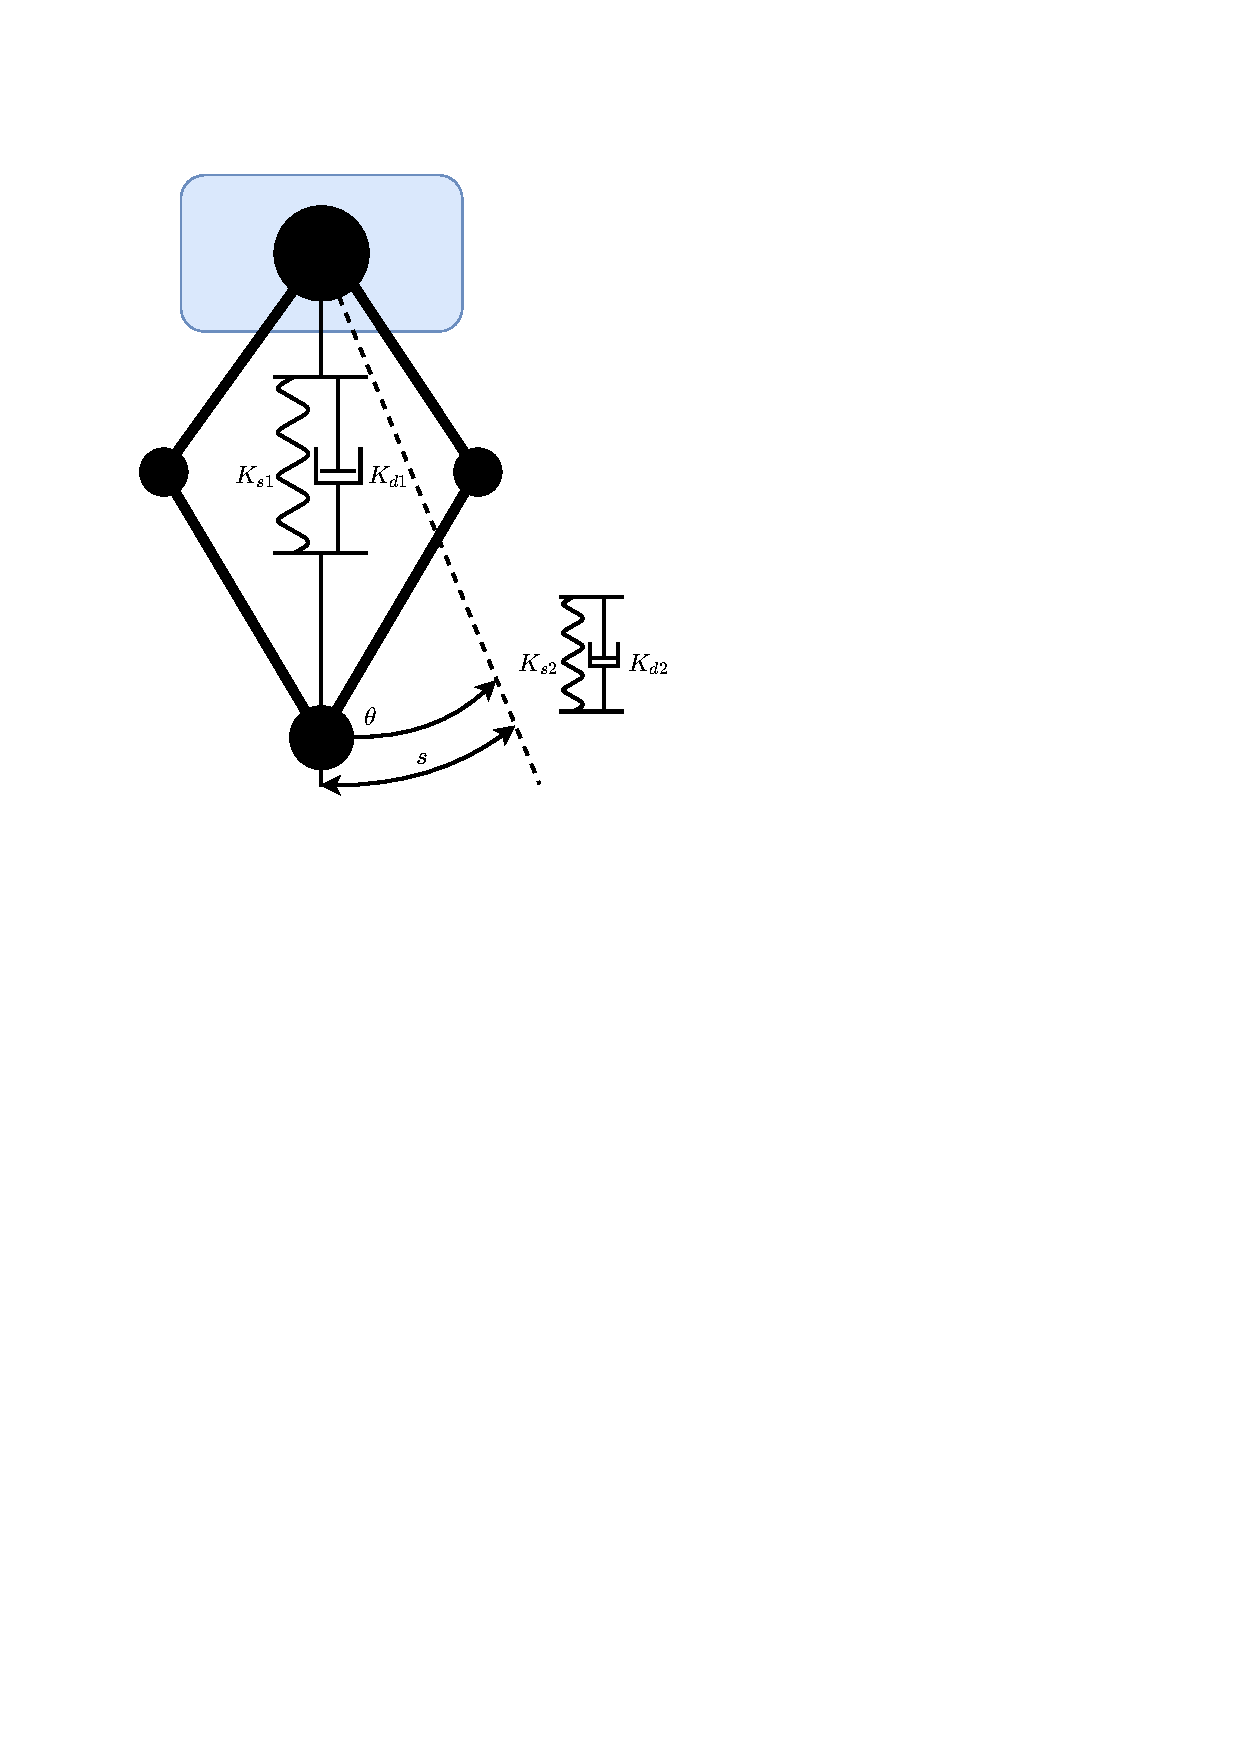
\includegraphics[clip, trim=2cm 15cm 9cm 2cm, page = 1, width=0.8\textwidth]{images/geometry/leg-spring-damper} 
\caption{Leg spring-damper virtual model.}
\label{fig:Leg spring-damper virtual model}
\end{figure}

\begin{figure}
\centering
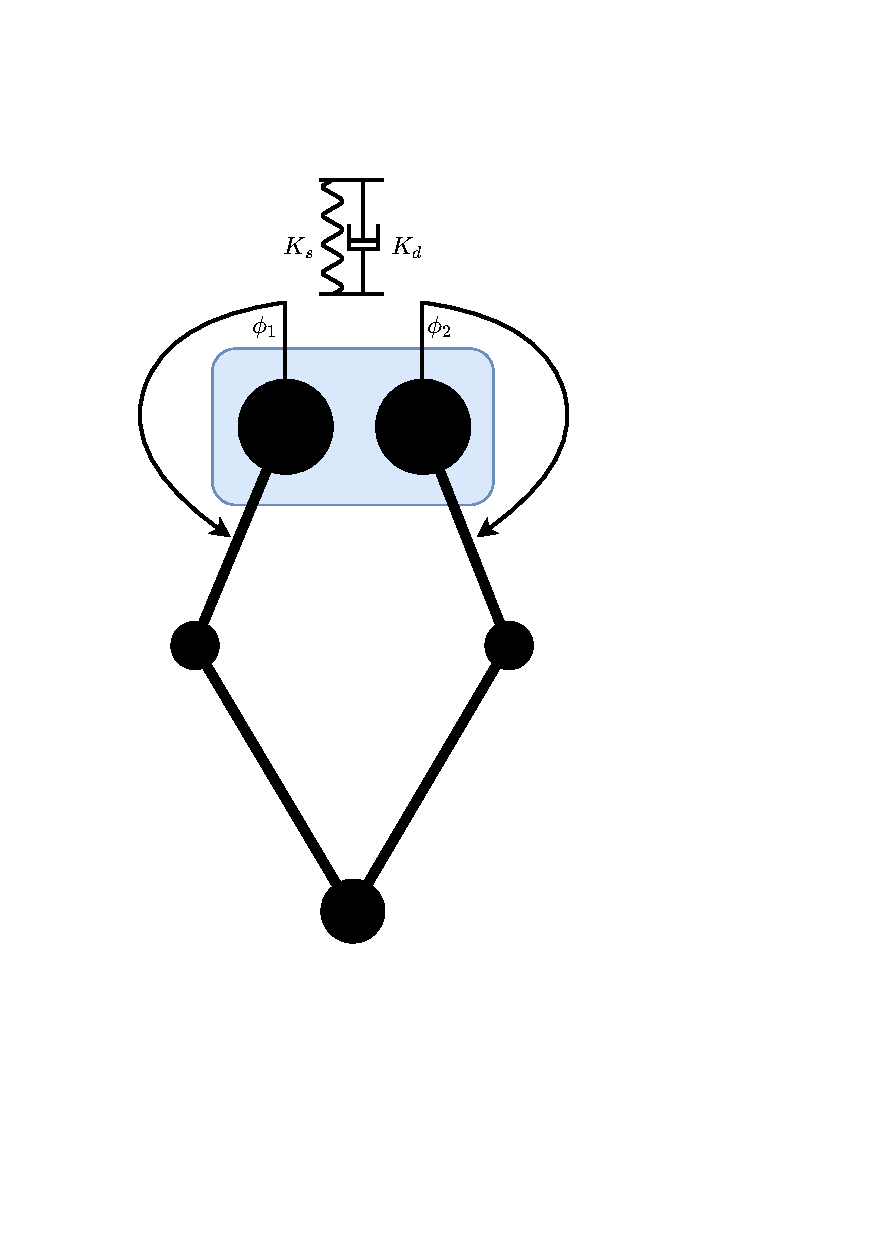
\includegraphics[clip, trim=2cm 12cm 10cm 2cm, page = 1, width=0.8\textwidth]{images/geometry/joint-spring-damper} 
\caption{Joint spring-damper virtual model.}
\label{fig:Joint spring-damper virtual model}
\end{figure}

\section{Spring-damper Mass Motion}
Using Newton's second law, the downward force of a mass under acceleration is:
\begin{equation}
F_m = ma = m\ddot{x}
\end{equation}

A spring with spring constant $k$ and a damper with damping constant $c$ have restoring forces as follows:
\begin{equation}
\begin{aligned}
&F_s = kx \\
&F_d = c\dot{x}
\end{aligned}
\end{equation}

Given the spring-damper mass system in \cref{fig:Spring-damper mass model}, free to oscillate, the equation of motion below is derived: 
\begin{equation}
\begin{aligned}
&-m\ddot{x} = kx + c\dot{x}\\
&m\ddot{x} + kx + c\dot{x} = 0
\end{aligned}
\end{equation}

By setting $x(t) = Ae^{\lambda t}$, the roots of the ODE above are:
\begin{equation} \label{eq:spring-damper-roots}
\lambda_{1,2} = \frac{-c \pm \sqrt{c^2 - 4mk}}{2m}
\end{equation}

\subsubsection{Critical Damping}
\begin{equation}
\begin{aligned}
&c^2 - 4mk = 0 \\
&c_{critical} = 2\sqrt{mk}
\end{aligned}
\end{equation}

\subsubsection{Damping Ratio}
\begin{equation}
\zeta = \frac{c}{c_{critical}}
\end{equation}
The equation \cref{eq:spring-damper-roots} can be restated in terms of the damping ratio as follows:
\begin{equation}
\lambda_{1,2} = (-\zeta \pm \sqrt{\zeta^2 - 1})\omega_0
\end{equation}

\subsubsection{Under, Over and Critical Damping}
For the spring-damper system to be under, over or critically damped, the following conditions must be met:
\begin{itemize}
\item Under: $\zeta < 1$ with imaginary roots
\item Over: $\zeta > 1$ 
\item Critical: $\zeta = 1$
\end{itemize}

For the robotic leg, ideally we want an under damped system when landing - this ensures some of the shock of landing is dissipated by the spring damper oscillations.

\subsubsection{Experimental Damping}
Experimentally the damping ratio $\zeta$ can be determined using the logarithmic decrement calculation. The logarithmic decrement is found by taking the natural logarithm of the ratio of amplitudes of two waveform peaks - this is then equated as follows:
\begin{equation}
\begin{aligned}
&\delta_n = ln(\frac{x_a}{x_{b}}) \\
&\zeta = \frac{\delta_n}{\sqrt{(2 \pi n)^2 + \delta_n^2}}
\end{aligned}
\end{equation}
where $n = b-a$ determines the number of peaks between measurements.

\subsubsection{Natural Frequency}
The natural frequency $\omega_0$ is the frequency the undamped system will oscillate at if given an initial $x$ offset and left to freely oscillate:
\begin{equation}
\omega_0 = \sqrt{\frac{k}{m}}\ [rad/s]
\end{equation}

The damped natural frequency is the same as above, but with the damping constant $c$ not equal to zero:
\begin{equation}
\omega_d = \sqrt{1 - \zeta^2}\omega_0\ [rad/s]
\end{equation}

\begin{figure}
\centering
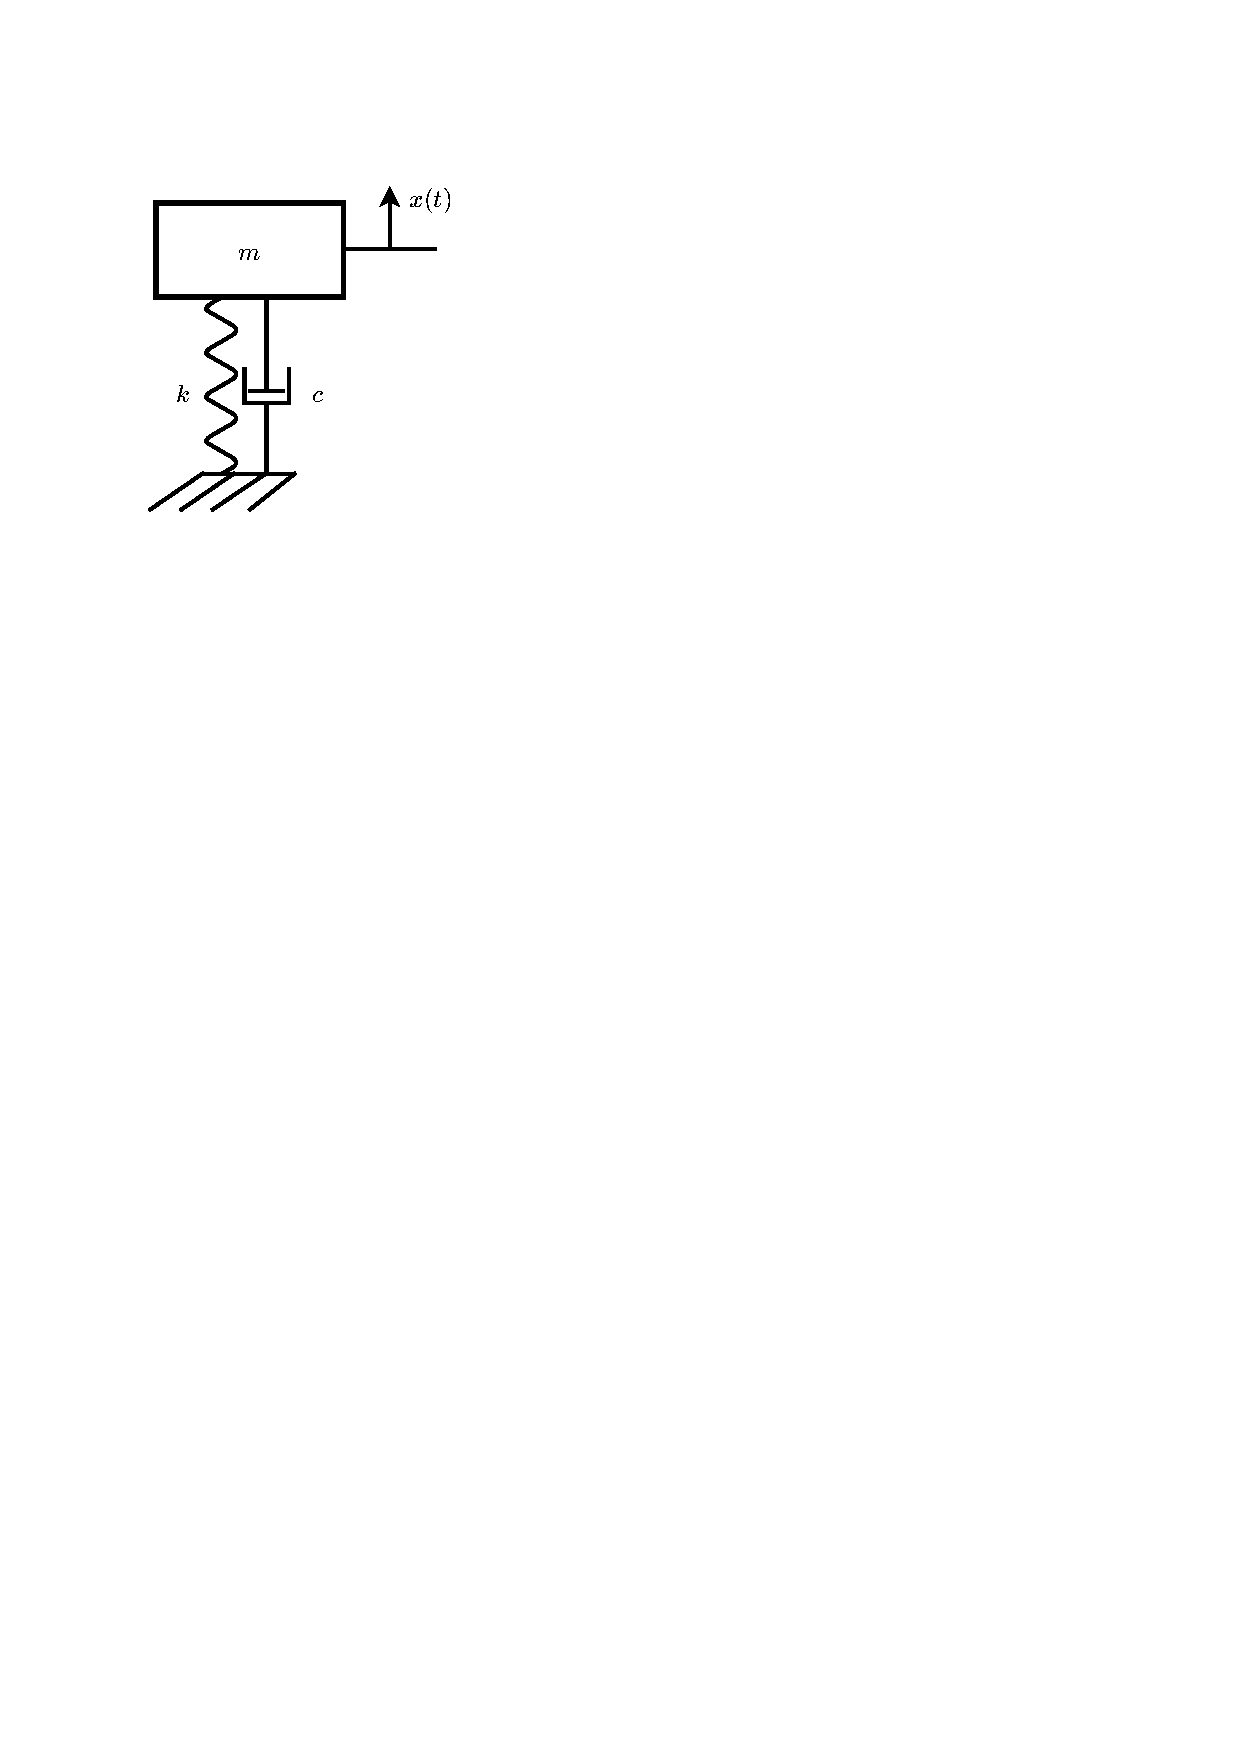
\includegraphics[clip, trim=2cm 20cm 13cm 2cm, page = 1, width=0.6\textwidth]{images/geometry/spring-damper-mass} 
\caption{Spring-damper mass model.}
\label{fig:Spring-damper mass model}
\end{figure}

\section{Leg Spring-damper Model}
\label{sec:Leg Spring-damper Model}
The leg, when viewed as a spring-damper mass system in free space, has a mass of approximately $0.5\ kg$ which is the mass of the leg linkages.

On impact and launching the leg spring-damper mass system is in contact with the ground and therefore the mass of the plate and motors acts on the entire system with a mass of approximately $2.2\ kg$.

\subsection{Impact Energy}
When the leg is dropped on the linear guide from its maximum height of $0.5\ m$ the potential energy that needs to be absorbed by the spring-damper is $10.791\ J$ as calculated in \cref{eq:spring-energy-drop}.
\begin{equation} \label{eq:spring-energy-drop}
\begin{aligned}
&E_p = mgh \\
&E_p = 2.2\times 9.81 \times 0.5 = 10.791\ J
\end{aligned}
\end{equation}

The spring-damper system should absorb all this energy with the leg depressed to a radial set-point of at most $0.3\ m$, to insure the body does not impact the ground. The majority of the impact energy will be absorbed as spring potential energy with the dynamics being changed slightly by the damper kinetic energy as seen in the spring-damper drop tests \cref{fig:spring-damper-tests}. The spring potential energy and damper kinetic energy are shown in \cref{eq:spring-damper-energy}.
\begin{equation} \label{eq:spring-damper-energy}
\begin{aligned}
&E_{ps} = \frac{1}{2}kx^2 \\
&E_{kd} = \frac{1}{2}c\dot{x}^2
\end{aligned}
\end{equation}

The velocity of the leg in free fall is approximately $2\ m/s$ found by performing drop tests and determining the number of video frames that it took for the leg to drop $0.4\ m$, which was approximately 5. Using \cref{eq:camera-frame-speed} the velocity was found.
\begin{equation} \label{eq:camera-frame-speed}
v_{final} = \frac{height}{frames \times \frac{1}{fps}} = \frac{0.4}{5 \times 0.04} = 2\ m/s
\end{equation}

A theoretical value for the spring constant $k$ can be found by using conservation of energy as seen in \cref{eq:spring-drop-energy-conservation}. A damping constant of $5\ N/(m/s)$ was assumed as determined through experimentation in \cref{fig:spring-damper-tests}.
\begin{equation} \label{eq:spring-drop-energy-conservation}
\begin{aligned}
&E_p = E_{ps} + E_{kd} \\
&mgh = \frac{1}{2}kx^2 + \frac{1}{2}c\dot{x}^2\\
&k = \frac{2(mgh - \frac{1}{2}c\dot{x}^2)}{x^2} = \frac{2(10.791 - \frac{1}{2}\times 5\times 2^2)}{(0.35-0.3)^2} = 632.8\ N/m
\end{aligned}
\end{equation}

\subsection{Launch Energy}
In order to launch the leg a set height of $0.4\ m$, the spring potential energy needs to be efficiently transferred into kinetic energy. This kinetic energy will launch the leg to a height with a corresponding potential energy. To calculate the spring constant needed to complete this jump assuming $80\ \%$ mechanical efficiency, equation \cref{eq:spring-launch-energy-conservation} is used. This is based on the principal of conservation of energy.

From \cref{eq:spring-damper-energy}, $E_{ps} = \frac{1}{2}k\Delta x^2$. Using an initial radial set-point of $0.3\ m$ and decompressing the spring to a radial set-point of $0.4\ m$ we get a $\delta x$ value of $-0.1\ m$.

\begin{equation} \label{eq:spring-launch-energy-conservation}
\begin{aligned}
&E_p = E_{ps} \\
&mgh = \frac{1}{2}k \Delta x^2 \\
&k = \frac{2mgh}{\Delta x^2} = \frac{2\times 2.2 \times 9.81 \times 0.4}{0.1^2} = 1726.6\ N/m
\end{aligned}
\end{equation}

\section{Virtual Compliance Model}

The following force vector provides a constant angular force, $f_{theta}$:
\begin{equation}
F = [f_r\ f_{\theta}]^T
\end{equation}

by using $f_{s}$, a force related to the arc-length of a polar system, the relation $s = r \theta$ exists:
\begin{equation}
F = [f_r\ f_{s}]^T
\end{equation}

\begin{equation}
f_a = k_s(a_{fbk} - a_{cmd}) + k_d(\dot{a}_{fbk} - \dot{a}_{cmd})
\end{equation}